\documentclass[11pt, letterpaper, includehead]{article}

%%%%%%%%%%%%%%%%%%%%% Pre-document %%%%%%%%%%%%%%%%%%%%%
\usepackage{fancyhdr}  % Allow for headers
\usepackage{graphicx}  % Allow for figures 
\usepackage{float}     % Allow for figure inserted in specified location
\usepackage{array}     % Allow for cell width manipulation
\usepackage{nicematrix}
\usepackage{multicol} % Multiple cols
\usepackage{tikz} % For latex graphics

\setlength{\parindent}{0pt} % Remove auto paragraph indents

% Get rid of those big ass margins
\usepackage[margin=1in]{geometry}

% Table cell formatting
\setlength{\arrayrulewidth}{0.25mm}
\setlength{\tabcolsep}{11pt}
\renewcommand{\arraystretch}{1.2}

\begin{document}

%%%%%%%%%%%%%%%%%%%%% Title Page %%%%%%%%%%%%%%%%%%%%%
\begin{titlepage}
  \begin{center}
    \Huge{\textbf{Lab 6}}\\
    \Huge{When Pigs Fly}
    \vfill
    \begin{figure}[H] % H makes the figure insert at the position in the document
      \centering
      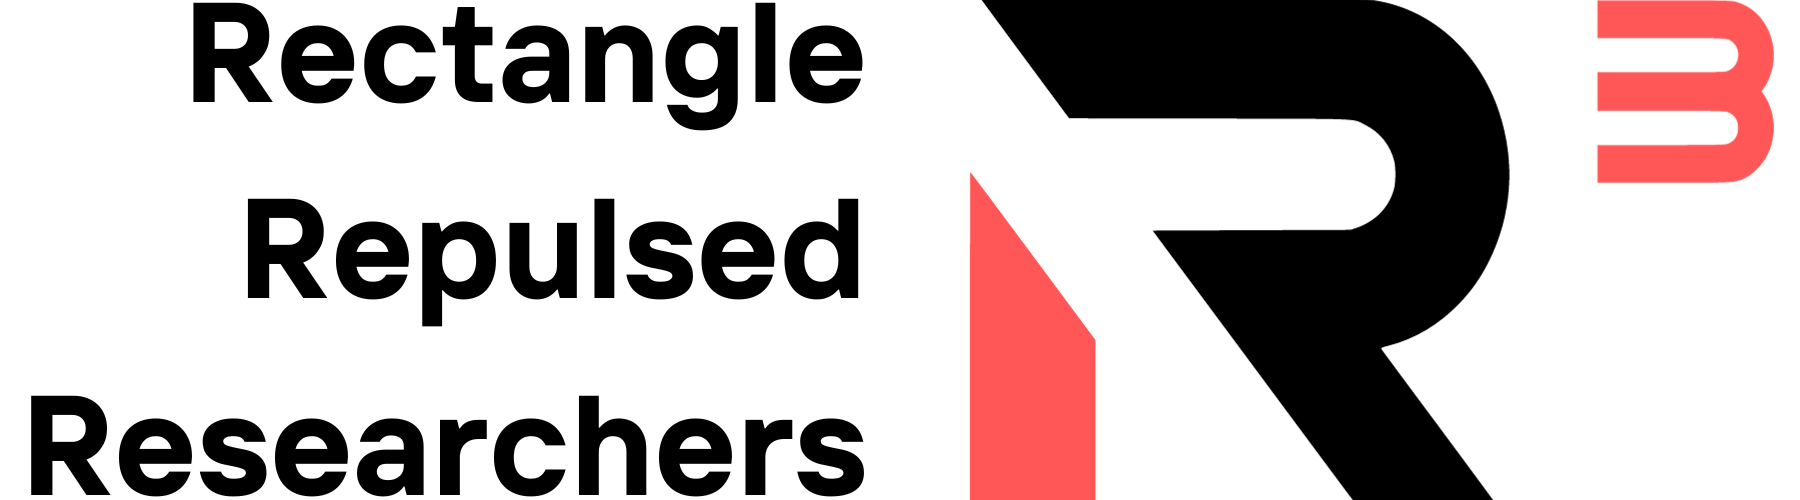
\includegraphics[width=6cm]{../logo.png}
    \end{figure}
    \large{\textbf{your name here}}\\
    \large{Julian Barossi, Liam Gilligan, Stephanie L'Heureux}\\
    \vspace{0.5cm}
    \normalsize
    \today
  \end{center}
\end{titlepage}

%%%%%%%%%%%%%%%%%%%%% TABLE OF CONTENTS %%%%%%%%%%%%%%%%%%%%%
\tableofcontents
\pagebreak % Move to next page

% Add a nice fancy header
\pagestyle{fancy}
\fancyhead{}
\fancyhead[C]{\textbf{Lab 5:} Forces and Acceleration}

%%%%%%%%%%%%%%%%%%%%%%%% SECTION 1 %%%%%%%%%%%%%%%%%%%%%%%%

\section{Set Up and Data Taking}


\renewcommand{\arraystretch}{2} 
\subsection{Measured values}
\begin{center}
  \begin{tabular}{|  m{5cm} | m{4cm} | m{3cm} | }
    \hline
    \textbf{Quantity} & \textbf{Value} & \textbf{SI units} \\
    \hline
    Mass  (m)  & $110.5g\left( \frac{1kg}{10^3g}\right)$ & $0.1105 kg$  \\
    \hline
    Diameter of cylinder ($\Delta x$) & $1in\left( \frac{0.0254m}{1in}\right)$ & $0.0254 m$  \\
    \hline
    Radius (r) & $48.25 cm \left( \frac{1m}{10^2cm}\right)$ & $0.4825 m$  \\
    \hline
  \end{tabular}
\end{center}
\renewcommand{\arraystretch}{1.5}

\section{Analyzing the Data}
\begin{center} 
  \begin{tabular}{|m{2.3cm}| m{1.7cm} | m{1.7cm} | m{2.4cm} | m{3.8cm} | m{1.2cm} |} 
    \hline
    \textbf{Tension (N)} & $\mathbf{F_{cent}}$ \textbf{(N)} & \textbf{Time (s)} & \textbf{Speed (m/s)} & \textbf{Expected Force (N)} & \textbf{\%diff}\\ 
    \hline
    1.28136 & 0.19846 & 0.0265139 & 0.9579880742 & 0.2101769888 & -5.57\%\\ 
    \hline
    1.26967 & 0.18677 & 0.0264788 & 0.9592579724 & 0.2107345747 & -11.4\%\\ 
    \hline
    1.27419 & 0.19129 & 0.0266464 & 0.9532244506 & 0.2080919633 & -8.07\%\\ 
    \hline
    1.27694 & 0.19404 & 0.0266976 & 0.9513963802 & 0.2072945813 & -6.39\%\\ 
    \hline
    1.26527 & 0.18237 & 0.0267601 & 0.9491743304 & 0.2063274114 & -11.6\%\\ 
    \hline
  \end{tabular} 
\end{center}
These values above were calculated with the methods detailed below, in which the values for the first column are found.
\subsection{Absolute value of the force}
The tension $T$ was found to be $1.28136N$ using the force sensor.

\subsection{Centripetal force from measured tension}
\begin{center}
  \begin{tikzpicture}
    \draw[thin,dashed][->] (-2,0) -- (2,0) node[right] {$x$}; % x axis
    \draw[thin,dashed][<-] (0,-2) -- (0,2) node[above] {$y$}; % y axis
    \draw[very thick, blue][->]  (0,0) --  node [right, pos=1, color=black] {$T$} (0,1.5); % tension
    \draw[very thick, blue][->]  (0,0) -- node [right, pos=1, color=black] {$mg$} (0,-1); % weight
    \draw[fill=black] (0,0) circle (0.08); % point in the center
  \end{tikzpicture}
\end{center}
$$\sum F_r = T - mg$$
$$\sum F_r = (1.28136N) - (0.1105 kg)(9.8 m/s^2)$$
$$\sum F_r = 0.19846N \approx 0.198N$$
$$\boxed{\sum F_r = 0.198N}$$

\subsection{Speed at the lowest point}


$$v = \frac{\Delta x}{t}$$
$$v = \frac{0.0254 m}{0.0265139s}$$
$$v = 0.9579880742...m/s \approx 0.958 m/s$$
$$\boxed{v = 0.958 m/s}$$

\subsection{Centripetal force from measured times}
\subsubsection{Calculations}
$$\sum F_r = ma_r$$
$$\sum F_r = (m)\left( \frac{v^2}{r}\right)$$
$$\sum F_r = (0.1105 kg)\left( \frac{(0.9579880742m/s)^2}{0.4825 m}\right)$$
$$\sum F_r = 0.21018...\approx 0.210N$$
$$\boxed{\sum F_r = 0.210N}$$

\subsubsection{Percent difference}
Let the force found using the tension be A and the force found using the time be B.
$$\%diff = \frac{F_{exp} - F_{thy}}{F_{thy}}\times 100\%$$
$$\%diff = \frac{0.198N - 0.210N}{0.210N}\times100\%$$
$$\%diff = -5.57\%$$

\subsection{Data from five recordings}
% The spread sheet is wrong lol

We suspected that the reason for the difference was likely due to the lack of fidelity
of the measuring aparatuses. We noticed in the graphs of the tension on the string over
time that it was quite jitterly, mostly (and inconveniently) at the troughs of the graph.
What's more, the change in time and change in position of the pendulum at the bottom were
fairly large, so the measurement of speed was likely decently inaccurate. Furhtermore, the 
time gate was not perfectly positioned at the bottom of the weight's swing, meaning that
even very accurate measurements of speed would have been measuring speed at the wrong location.

\section{When pigs fly}

\subsection{Free body diagram}
\begin{multicols}{2}
  \centering
  \begin{tikzpicture}
    \draw[thin,dashed][->] (-2,0) -- (2,0) node[right] {$x$}; % x axis
    \draw[thin,dashed][->] (0,-2) -- (0,2) node[above] {$y$}; % y axis
    \draw[very thick, blue][->]  (0,0) --  node [right, pos=1, color=black] {$T$} (1.5,1.5); % tension
    \draw[very thick, blue][->]  (0,0) -- node [right, pos=1, color=black] {$mg$} (0,-1.5); % weight
    \draw[fill=black] (0,0) circle (0.08); % point in the center
    \draw (0.7,0.7) arc (45:90:1);
    \draw (0,0.5) node[right] {$\theta$}; % point in the center
    % \draw (0,0) ++(0:2) arc (0:45:2); % point in the center
    % \draw[blue] (0,0) arc[start angle=-45, end angle=90, radius=1];
  \end{tikzpicture}

  \columnbreak

  \begin{tikzpicture}
    \draw[thin,dashed][->] (-2,0) -- (2,0) node[right] {$x$}; % x axis
    \draw[thin,dashed][->] (0,-2) -- (0,2) node[above] {$y$}; % y axis
    \draw[very thick, blue][->]  (0,0) --  node [below, pos=1, color=black] {$T\sin(\theta)$} (1,0); % tension
    \draw[very thick, blue][->]  (0,0) --  node [right, pos=1, color=black] {$T\cos(\theta)$} (0,1.5); % tension
    \draw[very thick, blue][->]  (0,0) -- node [right, pos=1, color=black] {$mg$} (0,-1.5); % weight
    \draw[fill=black] (0,0) circle (0.08);
  \end{tikzpicture}
\end{multicols}

\subsection{Derive equation of theoretical speed}
\begin{multicols}{2}
  \center{\textbf{x-axis}}
  $$\sum F_x = ma_x$$
  $$\sum F_x = \frac{mv^2}{r}$$
  $$T\sin(\theta) = \frac{mv^2}{r}$$

  \columnbreak
  \center{\textbf{y-axis}}
  $$\sum F_y = ma_y$$
  $$\sum F_y = 0$$
  $$T\cos\theta = mg$$
\end{multicols}

$$T\cos\theta = mg$$
$$T = \frac{mg}{\cos\theta}$$
$$T\sin\theta = \frac{mv^2}{r}$$
$$\frac{mg}{\cos\theta}\sin\theta = \frac{mv^2}{r}$$
$$mg\tan\theta = \frac{mv^2}{r}$$
$$v_{thy} = \sqrt{g \cdot r\tan\theta}$$\\\\
$$\tan\theta = \frac{opp}{adj} = \frac{r}{\sqrt{L^2-r^2}}$$\\\\
$$v_{thy} = \sqrt{g\cdot r\cdot\frac{r}{\sqrt{L^2-r^2}}}$$
$$\boxed{v_{thy} = \sqrt{\frac{g\cdot r^2}{\sqrt{L^2-r^2}}}}$$

\subsection{Theoretical speed}

$$v_{thy} = \sqrt{\frac{g\cdot r^2}{\sqrt{L^2-r^2}}}$$
$$v_{thy} = \sqrt{\frac{(9.80m/s^2)\cdot (0.605m)^2}{\sqrt{(0.97m)^2-(0.605m)^2}}}$$
$$\boxed{v_{thy} \approx 2.17508m/s}$$

\subsection{Measured values}

\renewcommand{\arraystretch}{2} 
\begin{center}
  \begin{tabular}{|  m{5cm} | m{4cm} | m{3cm} | }
    \hline
    \textbf{Quantity} & \textbf{Value} & \textbf{SI units} \\
    \hline
    Radius (r)  & $60.5 cm\left( \frac{1m}{10^2cm}\right)$ & $0.605 m$  \\
    \hline
    Length of string (L)  & $97 cm\left(\frac{1m}{10^2cm}\right)$ & $0.97m$ \\
    \hline
  \end{tabular}
\end{center}
\renewcommand{\arraystretch}{1.5}
For the period (T), we minimized human error by measuring the time for five revolutions then found the period 
by dividing by five. To further limit inaccuracies, this was repeated five times. For the period value, we 
took the average of these measurements.
\begin{center} 
  \begin{tabular}{|  m{2cm} | m{5cm} | m{5cm} | } 
    \hline
    \textbf{Attempt} & \textbf{Five revolutions (s)} & \textbf{One revolution (s)}\\ 
    \hline
    1 & 8.63 & 1.726 \\ 
    \hline
    2 & 8.68 & 1.736 \\ 
    \hline
    3 & 8.62 & 1.724 \\ 
    \hline
    4 & 8.61 & 1.722 \\ 
    \hline
    5 & 8.59 & 1.718 \\ 
    \hline
    \hline
    \multicolumn{2}{|l|}{{\textbf{Average period}}(\boldmath{$\bar{T}$})} & 1.7252 \\ 
    \hline  
  \end{tabular} 
\end{center} 

\subsection{Experimental speed}
$$v = \frac{2\pi r}{T}$$
$$v = \frac{2\pi (0.605 m)}{1.7252s}$$
$$v = \frac{1.21 \pi m}{1.7252s}$$
$$v = 2.203412421...m/s \approx  2.203m/s$$
$$\boxed{v_{exp} = 2.203m/s}$$

\subsection{Percent difference}
$$\%diff = \frac{v_{exp} - v_{thy}}{v_{thy}} \times 100\%$$
$$\%diff = \frac{2.203m/s - 2.17508m/s}{2.17508m/s} \times 100\%$$
$$\boxed{\%diff \approx 1.2836\%}$$

\end{document}
